% Career Navigator — Comprehensive Project Report
% Compile with: pdflatex (or use Overleaf)
\documentclass[12pt,a4paper]{report}

% ----- Packages -----
\usepackage[utf8]{inputenc}
\usepackage[T1]{fontenc}
\usepackage{graphicx}
\usepackage{hyperref}
\usepackage{float}
\usepackage{longtable}
\usepackage{enumitem}
\usepackage{tikz}
\usetikzlibrary{shapes,arrows,positioning,fit,backgrounds}
\usepackage{listings}
\usepackage{xcolor}
\usepackage{titlesec}
\usepackage{fancyhdr}
\usepackage{geometry}
\usepackage{booktabs}
\usepackage{tabularx}
\usepackage{caption}
\usepackage{amssymb}

\geometry{margin=1in}

% Code listing style
\definecolor{codegreen}{rgb}{0,0.6,0}
\definecolor{codegray}{rgb}{0.5,0.5,0.5}
\definecolor{codepurple}{rgb}{0.58,0,0.82}
\definecolor{backcolour}{rgb}{0.95,0.95,0.92}

\lstdefinestyle{mystyle}{
    backgroundcolor=\color{backcolour},
    commentstyle=\color{codegreen},
    keywordstyle=\color{magenta},
    numberstyle=\tiny\color{codegray},
    stringstyle=\color{codepurple},
    basicstyle=\ttfamily\footnotesize,
    breakatwhitespace=false,
    breaklines=true,
    captionpos=b,
    keepspaces=true,
    numbers=left,
    numbersep=5pt,
    showspaces=false,
    showstringspaces=false,
    showtabs=false,
    tabsize=2
}
\lstset{style=mystyle}

% Hyperlink setup
\hypersetup{
    colorlinks=true,
    linkcolor=blue,
    filecolor=magenta,
    urlcolor=cyan,
    pdftitle={Career Navigator — Project Report},
    pdfauthor={Career Navigator Team}
}

% Title formatting
\titleformat{\chapter}[display]
  {\normalfont\huge\bfseries}{\chaptertitlename\ \thechapter}{20pt}{\Huge}
\titlespacing*{\chapter}{0pt}{0pt}{20pt}

\begin{document}

% ============================================================
% TITLE PAGE
% ============================================================
\begin{titlepage}
\begin{center}

\vspace*{2cm}

{\Huge \textbf{Career Navigator}}\\[0.5cm]
{\Large An AI-Powered Career Guidance, Resume Building, and Job Matching Platform}\\[2cm]

{\large A Comprehensive Project Report}\\[1cm]


\includegraphics[width=4cm]{logo/logo.png}\\[2cm]

{\large \textbf{Department of Computer Science}}\\[0.3cm]
{\large \textbf{Faculty of Science}}\\[0.3cm]
{\large \textbf{[University Name]}}\\[2cm]

{\large \textbf{Team Members:}}\\[0.5cm]
{\large [Student 1 — Scrum Master]}\\[0.2cm]
{\large [Student 2 — Backend Developer]}\\[0.2cm]
{\large [Student 3 — Frontend Developer]}\\[0.2cm]
{\large [Student 4 — DevOps Engineer]}\\[0.2cm]
{\large [Student 5 — AI/ML Specialist]}\\[2cm]

{\large \textbf{Supervisor:} [Supervisor Name]}\\[1cm]

{\large \textbf{Date:} \today}

\end{center}
\end{titlepage}

% ============================================================
% TABLE OF CONTENTS
% ============================================================
\tableofcontents
\newpage

% ============================================================
% CHAPTER ONE: INTRODUCTION
% ============================================================
\chapter{Introduction}

\section{General Introduction}
The modern job market is characterized by rapid technological evolution, shifting industry demands, and an increasingly competitive global workforce. University students and early-career professionals face significant challenges in navigating their career paths — from identifying suitable job opportunities aligned with their skills, to crafting professional resumes, preparing for interviews, and connecting with mentors who can guide their professional development.

Career Navigator is an AI-powered, full-stack web application designed to bridge the gap between academic training and professional employment. The platform integrates intelligent career guidance, automated resume building from structured profile data, AI-driven CV parsing and skill extraction, job matching with relevance scoring, mentor discovery, real-time messaging, video calling capabilities for mock interviews, and an administrative analytics dashboard for monitoring platform engagement.

The system is built as a modern monorepo comprising a NestJS (TypeScript) REST API backend with Prisma ORM and PostgreSQL persistence, and a Next.js (React/TypeScript) frontend with Tailwind CSS styling and Framer Motion animations. Infrastructure is containerized via Docker and orchestrated with Kubernetes manifests for production deployment. The platform leverages Google Gemini and Ollama Cloud for AI capabilities including natural language chat restricted to career-path topics, mock interview simulations, course recommendations, and automated CV text extraction with structured skill identification.

\section{Aim and Objectives}

\subsection{Aim}
The primary aim of this project is to design and implement a comprehensive, AI-enhanced career development platform that empowers students and professionals to manage their career journey from a single integrated interface — from skill profiling and resume generation to job discovery, interview preparation, and mentor connection.

\subsection{Objectives}
The specific objectives of this project are:

\begin{enumerate}[label=\textbf{OBJ-\arabic*}:, leftmargin=*]
    \item To implement a secure authentication system using JWT access/refresh token rotation with OTP-based email verification and role-based access control (RBAC) for user and admin roles.
    \item To develop a structured user profile management system supporting personal details, education history, work experience, projects, references, and a flexible CV wizard for storing extensible resume data.
    \item To build an AI-powered resume/CV extraction pipeline using BullMQ job queues with Google Gemini as the primary AI provider and Ollama Cloud as fallback, capable of parsing PDF and DOCX documents and extracting structured data (skills, education, experience).
    \item To create a visual resume builder supporting six professionally designed A4 templates (Classic, Modern, Minimal, Creative, Professional, Executive) with print-to-PDF export functionality.
    \item To implement a job listings and matching system with AI-powered relevance reranking based on user skills extracted from their profile and CV.
    \item To develop a mentor discovery module enabling users to search for mentors by skills, expertise, and availability.
    \item To integrate real-time messaging via Socket.IO with Redis pub/sub for horizontal scaling, supporting one-on-one and group conversations.
    \item To implement AI chat functionality restricted to career-path topics with skill enforcement, mock interview simulations, and course recommendations across major online learning platforms.
    \item To integrate Agora video calling for live mock interview sessions with session metadata persistence.
    \item To build an administrative dashboard with user management, feedback moderation, and engagement analytics (KPIs: active jobs, total mentors, AI chats, total users).
    \item To containerize the entire system using Docker and provide Kubernetes deployment manifests for production orchestration.
    \item To implement comprehensive input validation, rate limiting, helmet security headers, CORS configuration, and file upload restrictions.
    \item To provide automated API documentation via Swagger/OpenAPI with bearer token authentication for interactive endpoint testing.
\end{enumerate}

\section{Problem Statement}
University graduates and job seekers in developing economies face a fragmented career development experience. They must navigate multiple disconnected platforms: job boards for opportunities, separate tools for resume building, external services for interview preparation, and informal networks for mentorship. This fragmentation leads to:

\begin{enumerate}[label=\textbf{P-\arabic*}:, leftmargin=*]
    \item \textbf{Disconnected career data}: User skills, education, and experience are scattered across different systems with no unified profile that feeds into job matching, resume generation, and skill gap analysis.
    \item \textbf{Time-consuming resume creation}: Manually formatting professional resumes for each job application is labor-intensive, and existing tools lack intelligent data population from verified user profiles and CV documents.
    \item \textbf{Limited AI-assisted career guidance}: Existing platforms either lack AI integration or provide generic AI responses without enforcing career-path relevance, leading to off-topic and unhelpful interactions.
    \item \textbf{Inefficient CV processing}: Recruiters and platforms still rely on manual CV review or basic keyword matching, missing the opportunity for AI-driven structured data extraction and skill identification.
    \item \textbf{Absence of integrated mentorship}: Job seekers lack a direct channel to connect with experienced professionals within the same platform ecosystem.
    \item \textbf{Lack of centralized analytics}: Educational institutions and career centers cannot track student career engagement metrics across platforms, limiting their ability to provide targeted support.
\end{enumerate}

Career Navigator addresses these problems by providing a unified, AI-enhanced platform that consolidates the entire career development workflow — from profile creation and CV parsing to job matching, interview practice, and mentor connection — within a single, secure, and scalable web application.

% ============================================================
% CHAPTER TWO: LITERATURE REVIEW
% ============================================================
\chapter{Literature Review}

\section{Software Development Methodologies}

\subsection{Waterfall Model}
The Waterfall model is a linear sequential approach where each phase must be completed before the next begins. Phases include requirements analysis, system design, implementation, testing, deployment, and maintenance. While straightforward and easy to understand, Waterfall lacks flexibility — changes introduced late in development are costly and difficult to accommodate. It is best suited for projects with well-defined, stable requirements.

\subsection{Agile Methodology}
Agile is an iterative approach emphasizing incremental delivery, customer collaboration, and responsiveness to change. Development occurs in short cycles (sprints) producing working software increments. The Agile Manifesto prioritizes individuals and interactions over processes, working software over comprehensive documentation, customer collaboration over contract negotiation, and responding to change over following a plan.

\subsection{Scrum Framework}
Scrum is an Agile framework that organizes work into fixed-length sprints (typically 2–4 weeks). Key roles include the Product Owner (manages backlog and prioritizes features), Scrum Master (facilitates process and removes impediments), and Development Team (self-organizing, cross-functional). Scrum ceremonies include Sprint Planning, Daily Stand-up, Sprint Review, and Sprint Retrospective. Artifacts include the Product Backlog, Sprint Backlog, and Increment.

\subsection{Kanban}
Kanban is a visual workflow management method emphasizing continuous delivery without fixed iterations. Work items are visualized on a Kanban board with columns representing workflow stages. Key practices include limiting work in progress (WIP), managing flow, making process policies explicit, and improving collaboratively.

\subsection{DevOps}
DevOps is a cultural and technical movement bridging development and operations teams. It emphasizes automation (CI/CD pipelines), continuous monitoring, infrastructure as code, and shared responsibility for production systems. DevOps practices complement Agile methodologies by enabling rapid, reliable software delivery.

\section{Comparison between different Software Development Methodologies}

\begin{table}[H]
\centering
\caption{Comparison of Software Development Methodologies}
\label{tab:methodology-comparison}
\begin{tabularx}{\textwidth}{|l|X|X|X|X|}
\hline
\textbf{Criterion} & \textbf{Waterfall} & \textbf{Scrum} & \textbf{Kanban} & \textbf{DevOps} \\
\hline
Approach & Sequential & Iterative & Continuous & Continuous \\
\hline
Flexibility & Low — rigid phases & High — adapts each sprint & High — continuous change & High — continuous delivery \\
\hline
Delivery & Single final release & Incremental (each sprint) & Continuous & Continuous \\
\hline
Team structure & Hierarchical & Cross-functional, self-organizing & Cross-functional & Cross-functional, DevOps culture \\
\hline
Customer involvement & At start and end only & Continuous (reviews) & On-demand & Continuous feedback \\
\hline
Risk management & Late discovery & Early and frequent & Continuous visibility & Automated testing/monitoring \\
\hline
Best for & Stable, well-defined requirements & Evolving requirements, complex products & Maintenance, support & Rapid deployment, microservices \\
\hline
\end{tabularx}
\end{table}

\section{Reason for the choice of Scrum Methodology}
For the Career Navigator project, the Scrum framework was selected for the following reasons:

\begin{enumerate}[label=\textbf{R-\arabic*}:, leftmargin=*]
    \item \textbf{Evolving requirements}: Career Navigator was developed incrementally across 8 milestones, each adding new features. Scrum's sprint-based approach allowed the team to reprioritize based on testing feedback and supervisor input after each sprint review.
    \item \textbf{Complex feature set}: With 13 distinct modules (auth, profile, resume, jobs, mentors, AI chat, video calling, realtime messaging, notifications, admin, courses, CV scanning, file uploads), breaking work into manageable sprints prevented scope creep and maintained team focus.
    \item \textbf{Cross-functional team}: The team comprised members with specialized skills (backend, frontend, DevOps, AI) who needed to collaborate closely. Daily stand-ups facilitated coordination and rapid issue resolution.
    \item \textbf{Risk mitigation}: Regular sprint reviews and retrospectives enabled early detection of integration issues (e.g., Docker build failures due to TypeScript errors, CV scan worker not starting) and allowed the team to course-correct before problems compounded.
    \item \textbf{Stakeholder visibility}: The Product Backlog and Sprint Backlog provided transparent tracking of completed, in-progress, and pending work, supporting grading evaluation based on individual contributions.
\end{enumerate}

\section{General review of related concepts with respect to Career Navigator}

\subsection{RESTful API Architecture}
Representational State Transfer (REST) is an architectural style for distributed hypermedia systems. Career Navigator implements REST principles through stateless HTTP endpoints organized by resource (auth, profile, jobs, mentors, etc.), using standard HTTP methods (GET, POST, PUT, PATCH, DELETE) and JSON as the data interchange format. Each endpoint is documented via Swagger/OpenAPI at \texttt{/api-docs}.

\subsection{Object-Oriented Programming (OOP) in NestJS}
NestJS leverages TypeScript's OOP features extensively. The four pillars of OOP are demonstrated throughout the codebase:
\begin{itemize}
    \item \textbf{Encapsulation}: Each service class (e.g., \texttt{AuthService}, \texttt{ProfileService}, \texttt{ResumeService}) encapsulates business logic and data access within well-defined method interfaces. Private methods handle internal operations while public methods expose the service contract.
    \item \textbf{Inheritance}: Controllers and services extend NestJS base classes. The \texttt{RedisIoAdapter} extends the default WebSocket adapter to add Redis pub/sub support.
    \item \textbf{Polymorphism}: The \texttt{UploadService} handles both profile pictures and CV files through a polymorphic \texttt{uploadToMinio} method parameterized by media type. The resume builder's \texttt{formatResume} method handles six different template types through a common data interface.
    \item \textbf{Abstraction}: The \texttt{PrismaService} abstracts database operations behind a clean interface. DTOs (Data Transfer Objects) abstract request validation using \texttt{class-validator} decorators.
\end{itemize}

\subsection{JWT Authentication and Authorization}
JSON Web Tokens (JWT) are used for stateless authentication. The system implements access token / refresh token rotation: short-lived access tokens (2 hours) authorize API requests, while longer-lived refresh tokens (30 days) are used to obtain new access tokens without re-login. Refresh tokens are stored hashed in the database with unique JTI (JWT ID) for revocation support. RBAC is enforced via a custom \texttt{RolesGuard} and \texttt{@Roles()} decorator.

\subsection{Prisma ORM and Database Design}
Prisma is a next-generation ORM providing type-safe database access. The Career Navigator data model comprises 20+ tables with relationships, indexes, and constraints defined declaratively in \texttt{schema.prisma}. Key design decisions include UUID primary keys, composite unique constraints (e.g., \texttt{[userId, type]} on upload media), cascade deletes for user-owned data, and JSON columns for flexible data storage (e.g., \texttt{cvWizardData} on profiles, \texttt{courses} on recommendation caches).

\subsection{Real-time Communication with WebSockets}
Socket.IO provides bidirectional, event-based communication between the web client and server. The \texttt{MessagingGateway} manages conversation rooms and broadcasts typing indicators and new message events. Redis is used as the Socket.IO adapter to synchronize events across multiple API instances for horizontal scaling.

\subsection{AI Integration — Gemini and Ollama}
The platform integrates two AI providers: Google Gemini (primary, via REST API with API key authentication) and Ollama Cloud (fallback, via OpenAI-compatible chat completions endpoint). The AI service enforces career-path relevance by deriving "allowed skills" from user data and validating model outputs. The CV scan worker uses Gemini for structured text extraction from PDF/DOCX documents with a 12-second timeout and automatic fallback to Ollama on failure.

\section{Review of related literature}

Several existing platforms and academic works have addressed aspects of the career development problem:

\begin{enumerate}[label=\textbf{L-\arabic*}:, leftmargin=*]
    \item \textbf{LinkedIn} (linkedin.com): The dominant professional networking platform providing profile hosting, job listings, and limited AI-powered job recommendations. However, it lacks integrated resume building with multiple templates, AI mock interviews, and direct mentor matching within the same interface.
    
    \item \textbf{Novoresume} (novoresume.com): A dedicated resume builder with professional templates and ATS optimization. It provides excellent resume formatting but lacks job matching, AI career chat, and mentor discovery features.
    
    \item \textbf{Zety} (zety.com): An online resume and cover letter builder with content suggestions. While strong in document creation, it does not integrate job search, skill gap analysis, or real-time career coaching.
    
    \item \textbf{Glassdoor} (glassdoor.com): Combines job listings with company reviews and salary insights. It provides valuable labor market data but does not offer AI-powered career guidance, resume generation, or mentorship connections.
    
    \item \textbf{Handshake} (joinhandshake.com): A career platform specifically for university students connecting them with employers. It focuses on early-career recruitment but lacks AI chat, CV parsing, and comprehensive resume template selection.
    
    \item \textbf{Academic Research}: Studies by Kenthapadi et al. (2017) on LinkedIn's job recommendation system demonstrate the value of machine learning for job-candidate matching. Research by Bian et al. (2020) on resume parsing using deep learning highlights the effectiveness of transformer-based models for structured information extraction from documents. Work by Gugnani and Misra (2020) on implicit skills extraction using word embeddings shows the potential of NLP techniques for skill identification from unstructured text.
\end{enumerate}

The Career Navigator project distinguishes itself by integrating all these capabilities — profile management, resume building, AI chat, CV parsing, job matching, mentorship, video calling, and analytics — into a single, cohesive platform with modern software engineering practices (microservices-ready architecture, containerization, CI/CD readiness, automated API documentation).

% ============================================================
% CHAPTER THREE: METHODOLOGY AND MATERIALS
% ============================================================
\chapter{Methodology and Materials}

\section{Research Methodology}
The development of Career Navigator followed an applied research methodology combining the Scrum agile framework with iterative prototyping. The methodology comprised five phases:

\begin{enumerate}[label=\textbf{Phase \arabic*}:, leftmargin=*]
    \item \textbf{Requirements Elicitation}: Analysis of existing career platforms, identification of gaps, and definition of functional and non-functional requirements. Stakeholder input was gathered from potential users (university students) and career counselors.
    
    \item \textbf{System Design}: High-Level Design (HLD) defining the multi-tier architecture (presentation, application, persistence, infrastructure layers). Low-Level Design including UML diagrams (use case, class, sequence) and database schema design.
    
    \item \textbf{Iterative Implementation}: Eight development sprints following the Scrum framework, each delivering a working increment of the system. Sprints were tracked via GitHub Projects with a Product Backlog and Sprint Backlogs.
    
    \item \textbf{Testing and Validation}: Unit testing (Jest), end-to-end testing (Supertest), manual smoke testing, and validation testing of input constraints (phone numbers, passwords, file uploads, URLs, emails).
    
    \item \textbf{Deployment and Documentation}: Docker containerization, Kubernetes manifest preparation, Swagger API documentation generation, and comprehensive project reporting.
\end{enumerate}

\section{System Requirements}

\subsection{Functional Requirements}

\begin{longtable}{|p{0.8cm}|p{6cm}|p{3cm}|p{3cm}|}
\hline
\textbf{ID} & \textbf{Requirement Description} & \textbf{Priority} & \textbf{Status} \\
\hline
FR-01 & User registration with email, password, and OTP verification (6-digit code, 10-minute expiry) & High & Implemented \\
\hline
FR-02 & JWT-based login with access token (2h) and refresh token (30d) rotation & High & Implemented \\
\hline
FR-03 & Password reset flow with OTP verification and new password confirmation & Medium & Implemented \\
\hline
FR-04 & Theme preference persistence (light/dark mode) per user & Low & Implemented \\
\hline
FR-05 & Profile CRUD — personal details (name, headline, phone, location, summary) & High & Implemented \\
\hline
FR-06 & CV Wizard — extensible JSON storage for skills, languages, interests, achievements, publications, etc. & High & Implemented \\
\hline
FR-07 & Education CRUD — degree, field of study, institution, start/end years, grade, description & High & Implemented \\
\hline
FR-08 & Work Experience CRUD — job title, company, location, start/end years, description & High & Implemented \\
\hline
FR-09 & Projects CRUD — title, description, external URL, skills array, active status & Medium & Implemented \\
\hline
FR-10 & References CRUD — name, relationship, company, email, phone, notes & Medium & Implemented \\
\hline
FR-11 & Profile picture upload (JPEG/PNG/WebP, max 5MB) to MinIO object storage & Medium & Implemented \\
\hline
FR-12 & CV upload (PDF/DOCX, max 10MB) with AI-powered text extraction and skill identification & High & Implemented \\
\hline
FR-13 & CV scan status polling — PENDING → PROCESSING → COMPLETED/FAILED & High & Implemented \\
\hline
FR-14 & Resume builder with 6 visual templates (Classic, Modern, Minimal, Creative, Professional, Executive) & High & Implemented \\
\hline
FR-15 & Resume generation from profile data + education + experience + projects + references & High & Implemented \\
\hline
FR-16 & Print-to-PDF export with A4 formatting and print-optimized CSS & High & Implemented \\
\hline
FR-17 & Job listings with search and pagination & High & Implemented \\
\hline
FR-18 & Job application with cover letter submission & High & Implemented \\
\hline
FR-19 & AI-powered job reranking based on user skills relevance & Medium & Implemented \\
\hline
FR-20 & Mentor discovery — search by skills, expertise & Medium & Implemented \\
\hline
FR-21 & AI chat — career-path-restricted conversation with skill enforcement & High & Implemented \\
\hline
FR-22 & AI mock interview — role-specific questions with difficulty levels & Medium & Implemented \\
\hline
FR-23 & AI course recommendations — Coursera, Simplilearn, edX, Udemy, Alison & Medium & Implemented \\
\hline
FR-24 & Real-time messaging — conversation creation, message sending, typing indicators via Socket.IO & High & Implemented \\
\hline
FR-25 & Notifications CRUD with mark-read functionality & Medium & Implemented \\
\hline
FR-26 & Agora video calling token generation and session management & Medium & Implemented \\
\hline
FR-27 & Admin user management — list users, update roles & High & Implemented \\
\hline
FR-28 & Admin feedback moderation — list feedback, update status & Medium & Implemented \\
\hline
FR-29 & Admin analytics dashboard — active jobs, total mentors, AI chats count, total users & Medium & Implemented \\
\hline
FR-30 & Swagger/OpenAPI documentation at /api-docs with bearer auth support & High & Implemented \\
\hline
\end{longtable}

\subsection{Non-Functional Requirements}

\begin{longtable}{|p{0.8cm}|p{5cm}|p{5cm}|p{2.5cm}|}
\hline
\textbf{ID} & \textbf{Requirement} & \textbf{Description} & \textbf{Status} \\
\hline
NFR-01 & Security & HTTPS/TLS, bcrypt password hashing, JWT token rotation, rate limiting, helmet headers, CORS configuration, RBAC enforcement & Implemented \\
\hline
NFR-02 & Performance & API response time < 500ms (95th percentile), BullMQ for async CV scanning, Redis caching for Socket.IO & Implemented \\
\hline
NFR-03 & Scalability & Horizontal scaling via Kubernetes HPA, Redis Socket.IO adapter for multi-instance WebSocket support & Implemented \\
\hline
NFR-04 & Reliability & Container health checks (Postgres, Redis, MinIO), automatic restart policies, database connection pooling & Implemented \\
\hline
NFR-05 & Maintainability & Modular NestJS architecture, TypeScript type safety, ESLint + Prettier code quality enforcement, monorepo structure & Implemented \\
\hline
NFR-06 & Portability & Docker containerization, Kubernetes deployment manifests, environment variable configuration & Implemented \\
\hline
NFR-07 & Usability & Responsive web UI (mobile + desktop), consistent dashboard layout, Framer Motion animations, toast notifications & Implemented \\
\hline
NFR-08 & Documentation & Swagger/OpenAPI auto-generated API docs, in-code JSDoc comments, README files, this comprehensive report & Implemented \\
\hline
NFR-09 & Testability & Jest unit tests, Supertest e2e tests, manual smoke test checklist & Implemented \\
\hline
NFR-10 & Availability & 99.9\% uptime target, graceful degradation when optional services are unavailable & Implemented \\
\hline
\end{longtable}

\section{System Design}

\subsection{High-Level Architecture (HLD)}

The Career Navigator system follows a multi-tier architecture with four distinct layers:

\begin{enumerate}[label=\textbf{Tier \arabic*}:, leftmargin=*]
    \item \textbf{Presentation Layer (Frontend)}: Next.js 16 (React 18) application with Tailwind CSS styling and Framer Motion animations. Runs on port 3000 (production) or 3002 (development). Communicates with the API layer via REST (JSON) and WebSockets (Socket.IO).
    
    \item \textbf{Application Layer (Backend API)}: NestJS 11 (TypeScript) application providing REST endpoints organized into 13 domain modules. Runs on port 3001 (development/production). Implements authentication, authorization, validation, business logic, and third-party integrations.
    
    \item \textbf{Persistence Layer}: PostgreSQL 16 (primary database via Prisma ORM), Redis 7 (caching, job queues, Socket.IO adapter), MinIO (object storage for profile pictures and CV files), OpenSearch (optional, for job search indexing).
    
    \item \textbf{Infrastructure Layer}: Docker Compose for local development and CI, Kubernetes (deployments, services, ingress) for production orchestration. External services include Google Gemini API, Ollama Cloud API, Agora Video SDK, and Brevo email API.
\end{enumerate}

\begin{figure}[H]
\centering
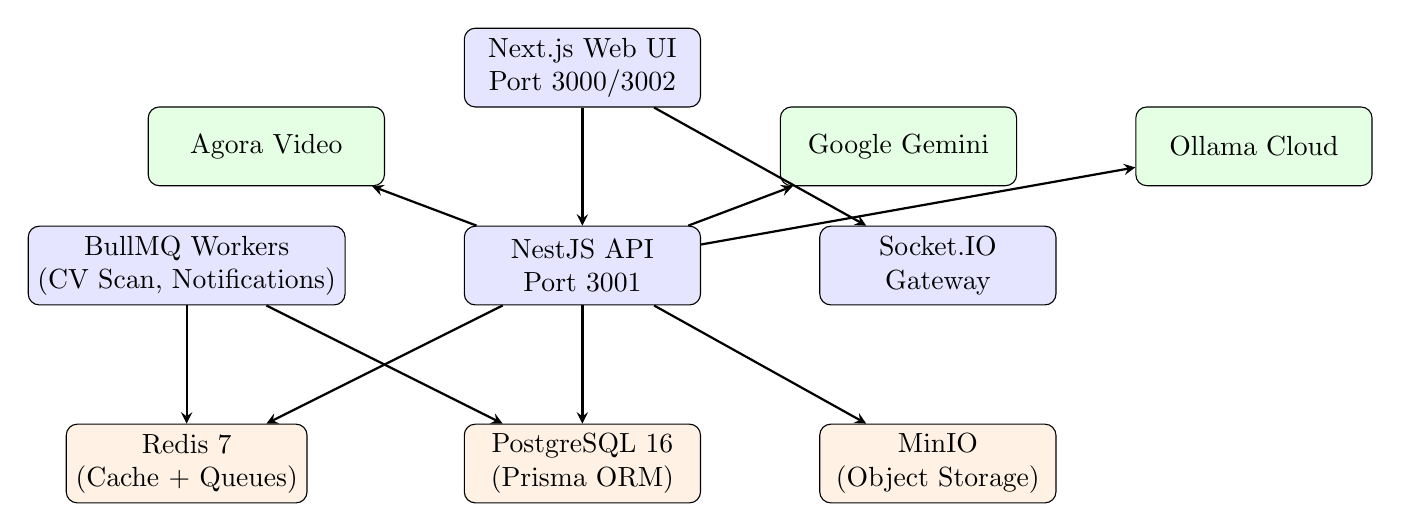
\begin{tikzpicture}[
    node distance=1.5cm,
    box/.style={rectangle, draw, rounded corners, minimum width=3cm, minimum height=1cm, align=center, fill=blue!10},
    infra/.style={rectangle, draw, rounded corners, minimum width=3cm, minimum height=1cm, align=center, fill=orange!10},
    ext/.style={rectangle, draw, rounded corners, minimum width=3cm, minimum height=1cm, align=center, fill=green!10},
    arrow/.style={->, >=stealth, thick}
]
    % Presentation Layer
    \node[box] (web) {Next.js Web UI\\Port 3000/3002};
    
    % Application Layer
    \node[box, below=of web] (api) {NestJS API\\Port 3001};
    \node[box, right=of api] (ws) {Socket.IO\\Gateway};
    \node[box, left=of api] (workers) {BullMQ Workers\\(CV Scan, Notifications)};
    
    % Persistence Layer
    \node[infra, below=of api] (pg) {PostgreSQL 16\\(Prisma ORM)};
    \node[infra, below=of workers] (redis) {Redis 7\\(Cache + Queues)};
    \node[infra, below=of ws] (minio) {MinIO\\(Object Storage)};
    
    % External Services
    \node[ext, above right=0.5cm and 1cm of api] (gemini) {Google Gemini};
    \node[ext, right=of gemini] (ollama) {Ollama Cloud};
    \node[ext, above left=0.5cm and 1cm of api] (agora) {Agora Video};
    
    % Arrows
    \draw[arrow] (web) -- (api);
    \draw[arrow] (web) -- (ws);
    \draw[arrow] (api) -- (pg);
    \draw[arrow] (api) -- (redis);
    \draw[arrow] (api) -- (minio);
    \draw[arrow] (workers) -- (redis);
    \draw[arrow] (workers) -- (pg);
    \draw[arrow] (api) -- (gemini);
    \draw[arrow] (api) -- (ollama);
    \draw[arrow] (api) -- (agora);
    
\end{tikzpicture}
\caption{High-Level Architecture Diagram}
\label{fig:hld}
\end{figure}

\subsection{UML Diagrams}

\subsubsection{Use Case Diagram}

\begin{figure}[H]
\centering
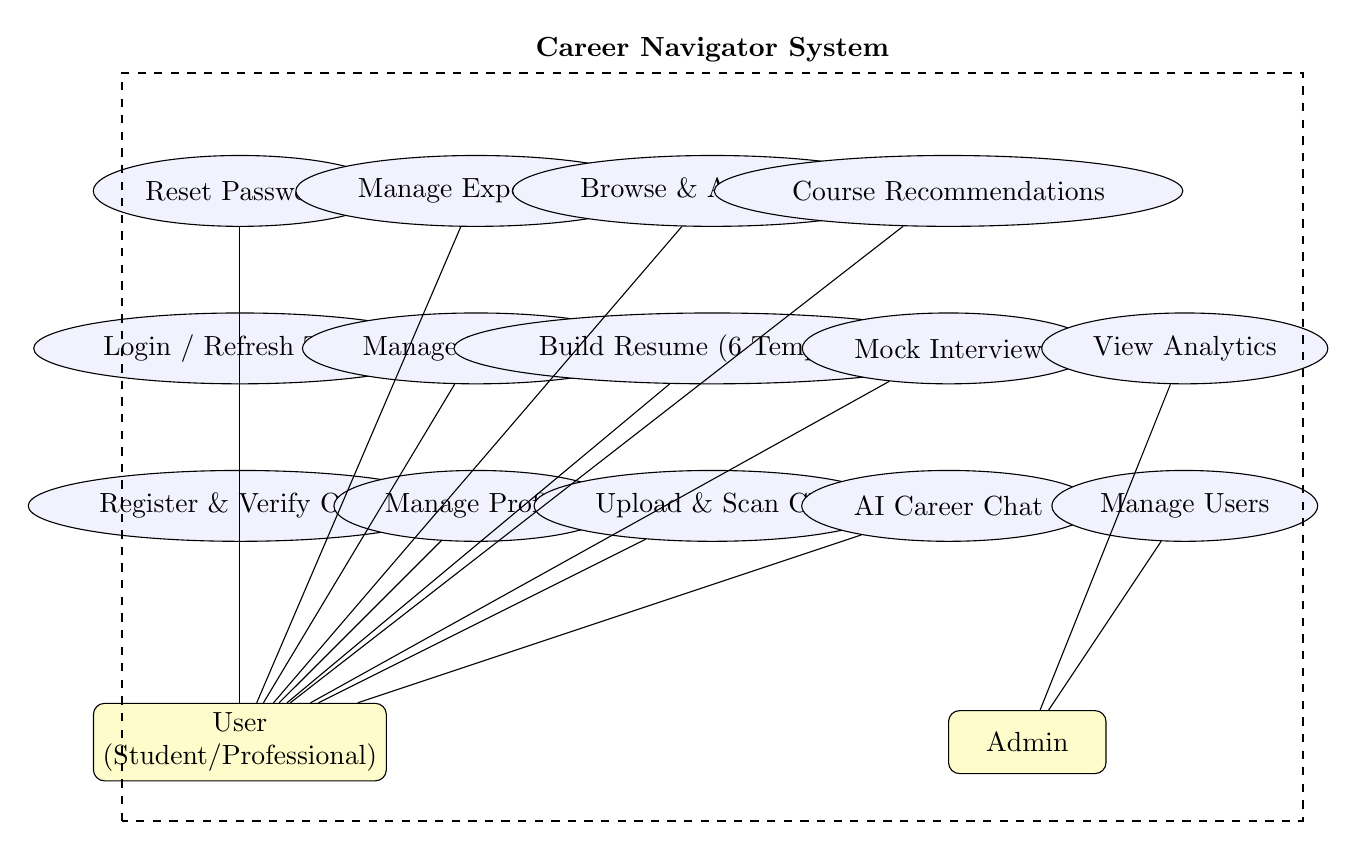
\begin{tikzpicture}[
    actor/.style={rectangle, draw, rounded corners, minimum width=2cm, minimum height=0.8cm, align=center, fill=yellow!20},
    usecase/.style={ellipse, draw, minimum width=2.5cm, minimum height=0.9cm, align=center, fill=blue!5},
]
    % Actors
    \node[actor] (user) at (0,0) {User\\(Student/Professional)};
    \node[actor] (admin) at (10,0) {Admin};
    
    % Use Cases - Auth
    \node[usecase] (register) at (0,3) {Register \& Verify OTP};
    \node[usecase] (login) at (0,5) {Login / Refresh Token};
    \node[usecase] (reset) at (0,7) {Reset Password};
    
    % Use Cases - Profile
    \node[usecase] (profile) at (3,3) {Manage Profile};
    \node[usecase] (education) at (3,5) {Manage Education};
    \node[usecase] (experience) at (3,7) {Manage Experience};
    
    % Use Cases - Core Features
    \node[usecase] (cvscan) at (6,3) {Upload \& Scan CV};
    \node[usecase] (resume) at (6,5) {Build Resume (6 Templates)};
    \node[usecase] (jobs) at (6,7) {Browse \& Apply Jobs};
    
    % Use Cases - AI
    \node[usecase] (aichat) at (9,3) {AI Career Chat};
    \node[usecase] (mock) at (9,5) {Mock Interview};
    \node[usecase] (courses) at (9,7) {Course Recommendations};
    
    % Admin Use Cases
    \node[usecase] (manageusers) at (12,3) {Manage Users};
    \node[usecase] (analytics) at (12,5) {View Analytics};
    
    % Connections
    \draw (user) -- (register);
    \draw (user) -- (login);
    \draw (user) -- (reset);
    \draw (user) -- (profile);
    \draw (user) -- (education);
    \draw (user) -- (experience);
    \draw (user) -- (cvscan);
    \draw (user) -- (resume);
    \draw (user) -- (jobs);
    \draw (user) -- (aichat);
    \draw (user) -- (mock);
    \draw (user) -- (courses);
    
    \draw (admin) -- (manageusers);
    \draw (admin) -- (analytics);
    
    % System boundary
    \draw[dashed, thick] (-1.5,-1) rectangle (13.5,8.5);
    \node at (6,8.8) {\textbf{Career Navigator System}};
    
\end{tikzpicture}
\caption{Use Case Diagram}
\label{fig:usecase}
\end{figure}

\subsubsection{Class Diagram (Core Domain Model)}

\begin{figure}[H]
\centering
\begin{tikzpicture}[
    class/.style={rectangle, draw, minimum width=4cm, minimum height=0.6cm, align=left, fill=blue!3},
    arrow/.style={->, >=open triangle 90}
]
    % User class
    \node[class, minimum height=4cm] (user) at (0,0) {
        \textbf{User}\\
        \hline
        + id: string (UUID)\\
        + email: string\\
        + passwordHash: string\\
        + isActive: boolean\\
        + role: UserRole (USER|ADMIN)\\
        + themePreference: ThemePreference\\
        \hline
        + profile: Profile?\\
        + educations: Education[]\\
        + workExperiences: WorkExperience[]\\
    };
    
    % Profile class
    \node[class, minimum height=3cm] (profile) at (5,-1) {
        \textbf{Profile}\\
        \hline
        + firstName: string?\\
        + lastName: string?\\
        + headline: string?\\
        + phone: string?\\
        + location: string?\\
        + summary: string?\\
        + cvWizardData: Json?\\
        \hline
    };
    
    % Education class
    \node[class, minimum height=1.5cm] (edu) at (5,3) {
        \textbf{Education}\\
        \hline
        + degree, fieldOfStudy, institution: string?\\
        + startYear, endYear: Int?\\
        + grade, description: string?\\
        + isCurrent: boolean\\
    };
    
    % WorkExperience class
    \node[class, minimum height=1.5cm] (work) at (10,3) {
        \textbf{WorkExperience}\\
        \hline
        + jobTitle, company, location: string?\\
        + startYear, endYear: Int?\\
        + description: string?\\
        + isCurrent: boolean\\
    };
    
    % Relationships
    \draw[arrow] (user) -- (profile) node[midway, above] {1:1};
    \draw[arrow] (user) -- (edu) node[midway, above] {1:N};
    \draw[arrow] (user) -- (work) node[midway, above] {1:N};
    
\end{tikzpicture}
\caption{Class Diagram — Core Domain Model}
\label{fig:class}
\end{figure}

\subsubsection{Object Diagram — Sample User Profile}

\begin{figure}[H]
\centering
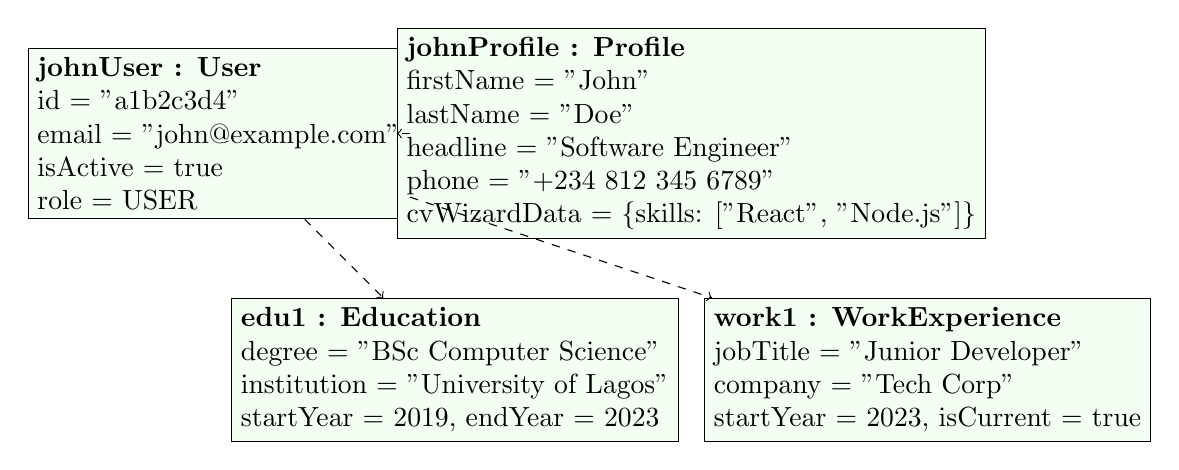
\begin{tikzpicture}[
    obj/.style={rectangle, draw, minimum width=4.5cm, align=left, fill=green!5}
]
    \node[obj] (john) at (0,0) {
        \textbf{johnUser : User}\\
        id = "a1b2c3d4"\\
        email = "john@example.com"\\
        isActive = true\\
        role = USER
    };
    
    \node[obj] (johnProfile) at (6,0) {
        \textbf{johnProfile : Profile}\\
        firstName = "John"\\
        lastName = "Doe"\\
        headline = "Software Engineer"\\
        phone = "+234 812 345 6789"\\
        cvWizardData = \{skills: ["React", "Node.js"]\}
    };
    
    \node[obj] (edu1) at (3,-3) {
        \textbf{edu1 : Education}\\
        degree = "BSc Computer Science"\\
        institution = "University of Lagos"\\
        startYear = 2019, endYear = 2023
    };
    
    \node[obj] (work1) at (9,-3) {
        \textbf{work1 : WorkExperience}\\
        jobTitle = "Junior Developer"\\
        company = "Tech Corp"\\
        startYear = 2023, isCurrent = true
    };
    
    \draw[->, dashed] (john) -- (johnProfile);
    \draw[->, dashed] (john) -- (edu1);
    \draw[->, dashed] (john) -- (work1);
    
\end{tikzpicture}
\caption{Object Diagram — Sample User Profile Instance}
\label{fig:object}
\end{figure}

\subsubsection{Sequence Diagrams}

\textbf{Sequence Diagram 1: User Registration with OTP Verification}

\begin{figure}[H]
\centering
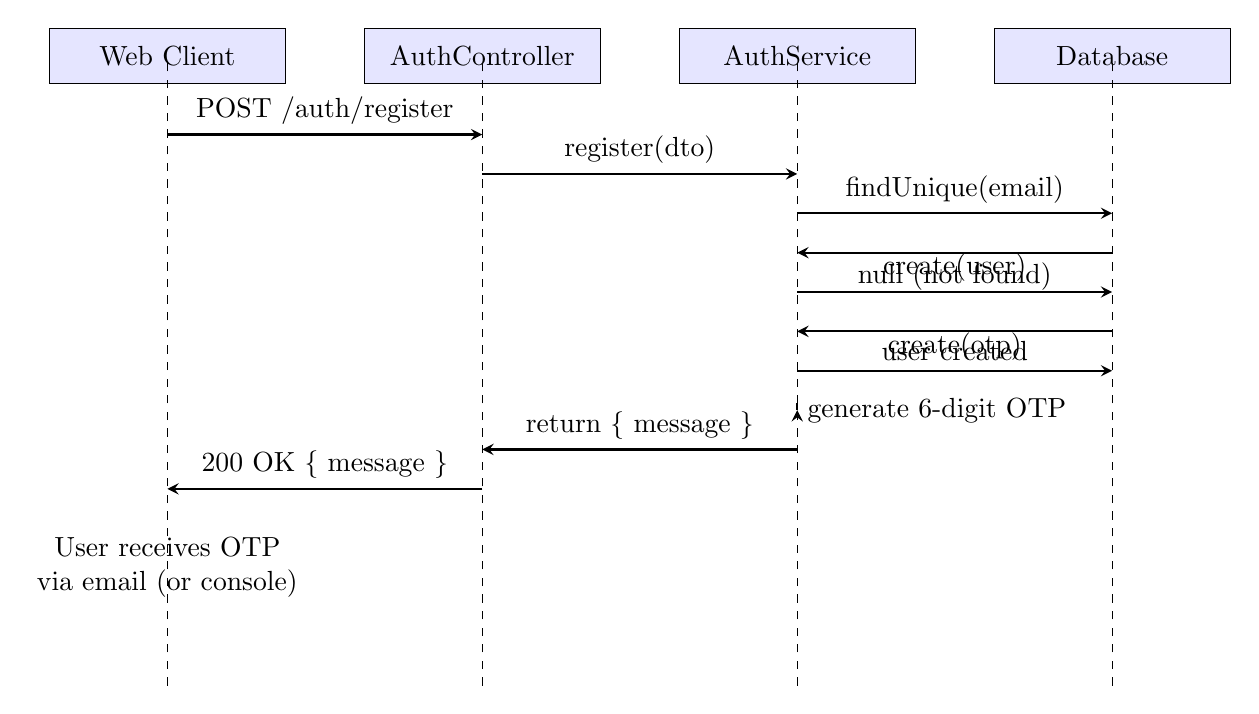
\begin{tikzpicture}[
    lifeline/.style={rectangle, draw, minimum width=3cm, minimum height=0.7cm, align=center, fill=blue!10},
    msg/.style={->, >=stealth, thick},
    selfmsg/.style={->, >=stealth, thick, loop right}
]
    % Lifelines
    \node[lifeline] (client) at (0,8) {Web Client};
    \node[lifeline] (api) at (4,8) {AuthController};
    \node[lifeline] (svc) at (8,8) {AuthService};
    \node[lifeline] (db) at (12,8) {Database};

    \draw[dashed] (0,0) -- (0,8);
    \draw[dashed] (4,0) -- (4,8);
    \draw[dashed] (8,0) -- (8,8);
    \draw[dashed] (12,0) -- (12,8);

    % Messages
    \draw[msg] (0,7) -- (4,7) node[midway, above] {POST /auth/register};
    \draw[msg] (4,6.5) -- (8,6.5) node[midway, above] {register(dto)};
    \draw[msg] (8,6) -- (12,6) node[midway, above] {findUnique(email)};
    \draw[msg] (12,5.5) -- (8,5.5) node[midway, below] {null (not found)};
    \draw[msg] (8,5) -- (12,5) node[midway, above] {create(user)};
    \draw[msg] (12,4.5) -- (8,4.5) node[midway, below] {user created};
    \draw[msg] (8,4) -- (12,4) node[midway, above] {create(otp)};
    \draw[msg] (8,3.5) -- (8,3.5) node[right] {generate 6-digit OTP};
    \draw[msg] (8,3) -- (4,3) node[midway, above] {return \{ message \}};
    \draw[msg] (4,2.5) -- (0,2.5) node[midway, above] {200 OK \{ message \}};

    \node at (0,1.5) [align=center] {User receives OTP\\via email (or console)};
\end{tikzpicture}
\caption{Sequence Diagram — User Registration with OTP}
\label{fig:seq1}
\end{figure}

\textbf{Sequence Diagram 2: CV Upload and AI Scan}

\begin{figure}[H]
\centering
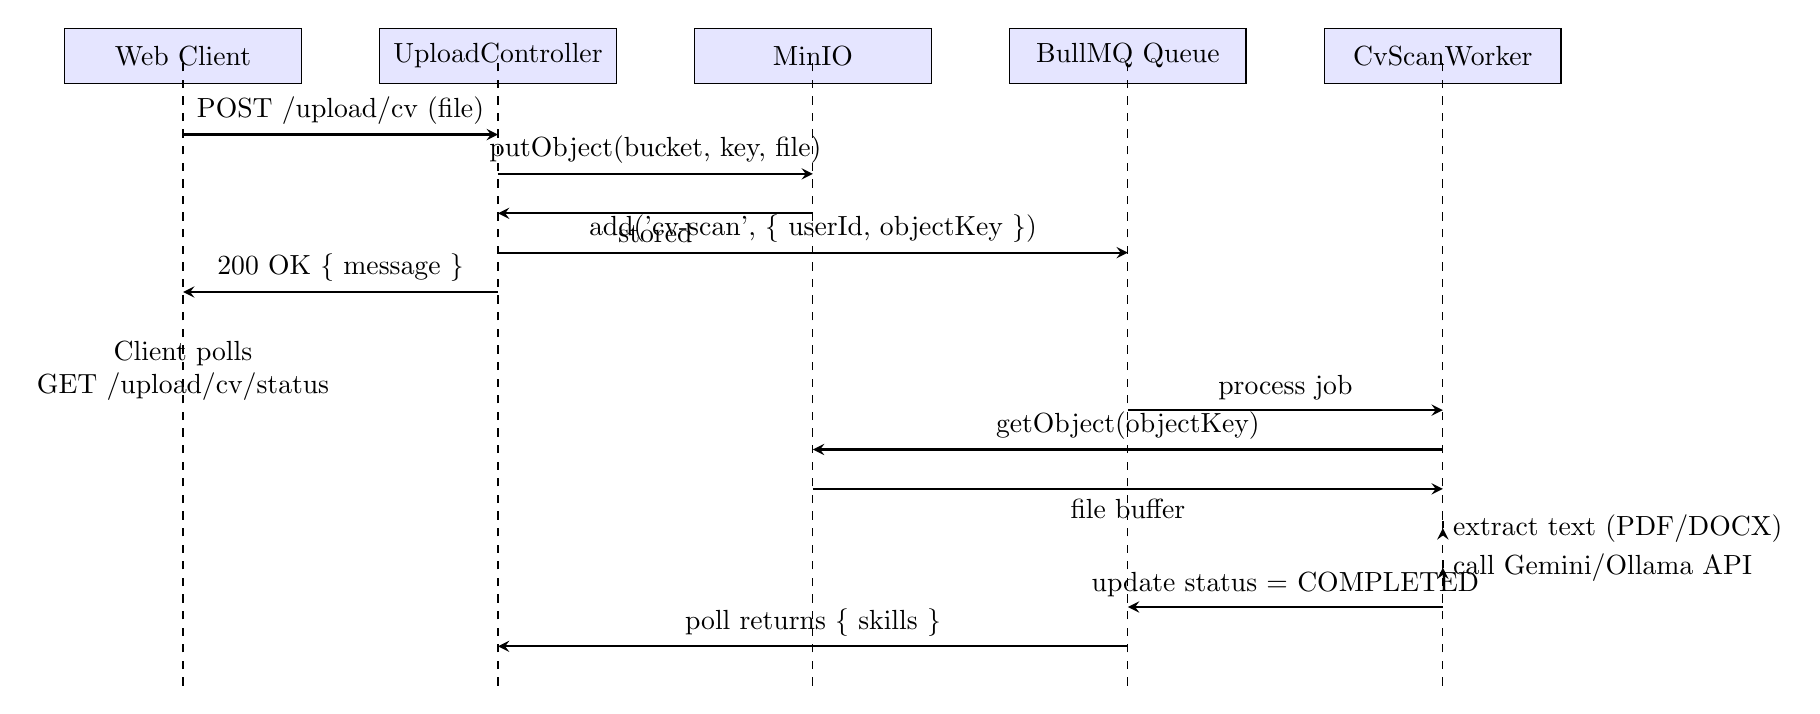
\begin{tikzpicture}[
    lifeline/.style={rectangle, draw, minimum width=3cm, minimum height=0.7cm, align=center, fill=blue!10},
    msg/.style={->, >=stealth, thick}
]
    \node[lifeline] (client) at (0,8) {Web Client};
    \node[lifeline] (upload) at (4,8) {UploadController};
    \node[lifeline] (minio) at (8,8) {MinIO};
    \node[lifeline] (queue) at (12,8) {BullMQ Queue};
    \node[lifeline] (worker) at (16,8) {CvScanWorker};

    \draw[dashed] (0,0) -- (0,8);
    \draw[dashed] (4,0) -- (4,8);
    \draw[dashed] (8,0) -- (8,8);
    \draw[dashed] (12,0) -- (12,8);
    \draw[dashed] (16,0) -- (16,8);

    \draw[msg] (0,7) -- (4,7) node[midway, above] {POST /upload/cv (file)};
    \draw[msg] (4,6.5) -- (8,6.5) node[midway, above] {putObject(bucket, key, file)};
    \draw[msg] (8,6) -- (4,6) node[midway, below] {stored};
    \draw[msg] (4,5.5) -- (12,5.5) node[midway, above] {add('cv-scan', \{ userId, objectKey \})};
    \draw[msg] (4,5) -- (0,5) node[midway, above] {200 OK \{ message \}};
    
    \node at (0,4) [align=center] {Client polls\\GET /upload/cv/status};
    
    \draw[msg] (12,3.5) -- (16,3.5) node[midway, above] {process job};
    \draw[msg] (16,3) -- (8,3) node[midway, above] {getObject(objectKey)};
    \draw[msg] (8,2.5) -- (16,2.5) node[midway, below] {file buffer};
    \draw[msg] (16,2) -- (16,2) node[right] {extract text (PDF/DOCX)};
    \draw[msg] (16,1.5) -- (16,1.5) node[right] {call Gemini/Ollama API};
    \draw[msg] (16,1) -- (12,1) node[midway, above] {update status = COMPLETED};
    \draw[msg] (12,0.5) -- (4,0.5) node[midway, above] {poll returns \{ skills \}};
\end{tikzpicture}
\caption{Sequence Diagram — CV Upload and AI-Powered Scan}
\label{fig:seq2}
\end{figure}

\textbf{Sequence Diagram 3: Resume Building Workflow}

\begin{figure}[H]
\centering
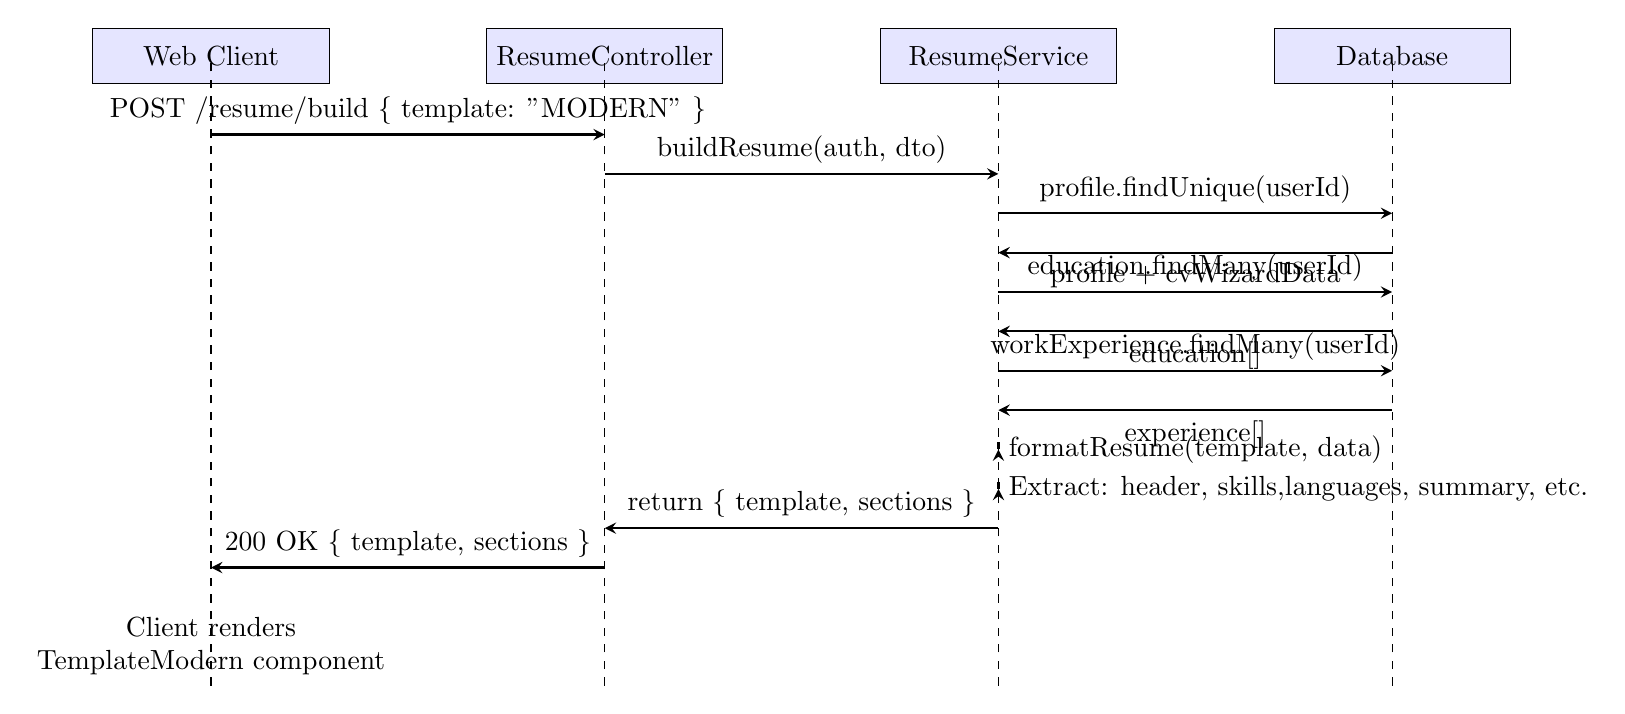
\begin{tikzpicture}[
    lifeline/.style={rectangle, draw, minimum width=3cm, minimum height=0.7cm, align=center, fill=blue!10},
    msg/.style={->, >=stealth, thick}
]
    \node[lifeline] (client) at (0,8) {Web Client};
    \node[lifeline] (resume) at (5,8) {ResumeController};
    \node[lifeline] (svc) at (10,8) {ResumeService};
    \node[lifeline] (db) at (15,8) {Database};

    \draw[dashed] (0,0) -- (0,8);
    \draw[dashed] (5,0) -- (5,8);
    \draw[dashed] (10,0) -- (10,8);
    \draw[dashed] (15,0) -- (15,8);

    \draw[msg] (0,7) -- (5,7) node[midway, above] {POST /resume/build \{ template: "MODERN" \}};
    \draw[msg] (5,6.5) -- (10,6.5) node[midway, above] {buildResume(auth, dto)};
    
    \draw[msg] (10,6) -- (15,6) node[midway, above] {profile.findUnique(userId)};
    \draw[msg] (15,5.5) -- (10,5.5) node[midway, below] {profile + cvWizardData};
    
    \draw[msg] (10,5) -- (15,5) node[midway, above] {education.findMany(userId)};
    \draw[msg] (15,4.5) -- (10,4.5) node[midway, below] {education[]};
    
    \draw[msg] (10,4) -- (15,4) node[midway, above] {workExperience.findMany(userId)};
    \draw[msg] (15,3.5) -- (10,3.5) node[midway, below] {experience[]};
    
    \draw[msg] (10,3) -- (10,3) node[right] {formatResume(template, data)};
    \draw[msg] (10,2.5) -- (10,2.5) node[right] {Extract: header, skills,\\languages, summary, etc.};
    
    \draw[msg] (10,2) -- (5,2) node[midway, above] {return \{ template, sections \}};
    \draw[msg] (5,1.5) -- (0,1.5) node[midway, above] {200 OK \{ template, sections \}};
    
    \node at (0,0.5) [align=center] {Client renders\\TemplateModern component};
\end{tikzpicture}
\caption{Sequence Diagram — Resume Building}
\label{fig:seq3}
\end{figure}

\textbf{Sequence Diagram 4: Real-Time Messaging via Socket.IO}

\begin{figure}[H]
\centering
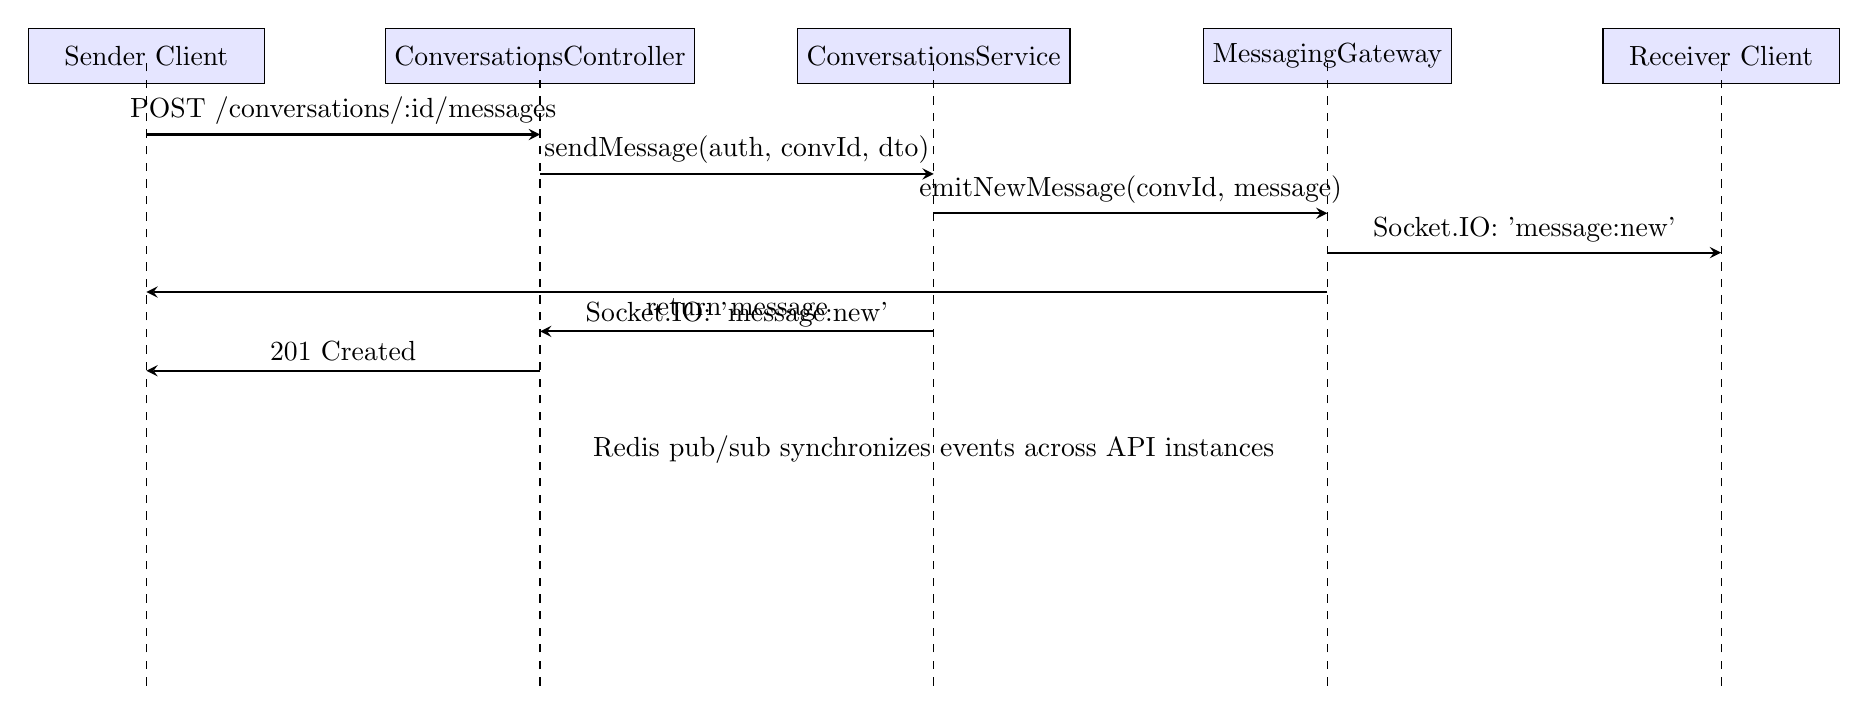
\begin{tikzpicture}[
    lifeline/.style={rectangle, draw, minimum width=3cm, minimum height=0.7cm, align=center, fill=blue!10},
    msg/.style={->, >=stealth, thick}
]
    \node[lifeline] (sender) at (0,8) {Sender Client};
    \node[lifeline] (api) at (5,8) {ConversationsController};
    \node[lifeline] (svc) at (10,8) {ConversationsService};
    \node[lifeline] (gateway) at (15,8) {MessagingGateway};
    \node[lifeline] (receiver) at (20,8) {Receiver Client};

    \draw[dashed] (0,0) -- (0,8);
    \draw[dashed] (5,0) -- (5,8);
    \draw[dashed] (10,0) -- (10,8);
    \draw[dashed] (15,0) -- (15,8);
    \draw[dashed] (20,0) -- (20,8);

    \draw[msg] (0,7) -- (5,7) node[midway, above] {POST /conversations/:id/messages};
    \draw[msg] (5,6.5) -- (10,6.5) node[midway, above] {sendMessage(auth, convId, dto)};
    \draw[msg] (10,6) -- (15,6) node[midway, above] {emitNewMessage(convId, message)};
    \draw[msg] (15,5.5) -- (20,5.5) node[midway, above] {Socket.IO: 'message:new'};
    \draw[msg] (15,5) -- (0,5) node[midway, below] {Socket.IO: 'message:new'};
    \draw[msg] (10,4.5) -- (5,4.5) node[midway, above] {return message};
    \draw[msg] (5,4) -- (0,4) node[midway, above] {201 Created};

    \node at (10,3) {Redis pub/sub synchronizes events across API instances};
\end{tikzpicture}
\caption{Sequence Diagram — Real-Time Messaging}
\label{fig:seq4}
\end{figure}

\textbf{Sequence Diagram 5: AI Chat with Career-Path Enforcement}

\begin{figure}[H]
\centering
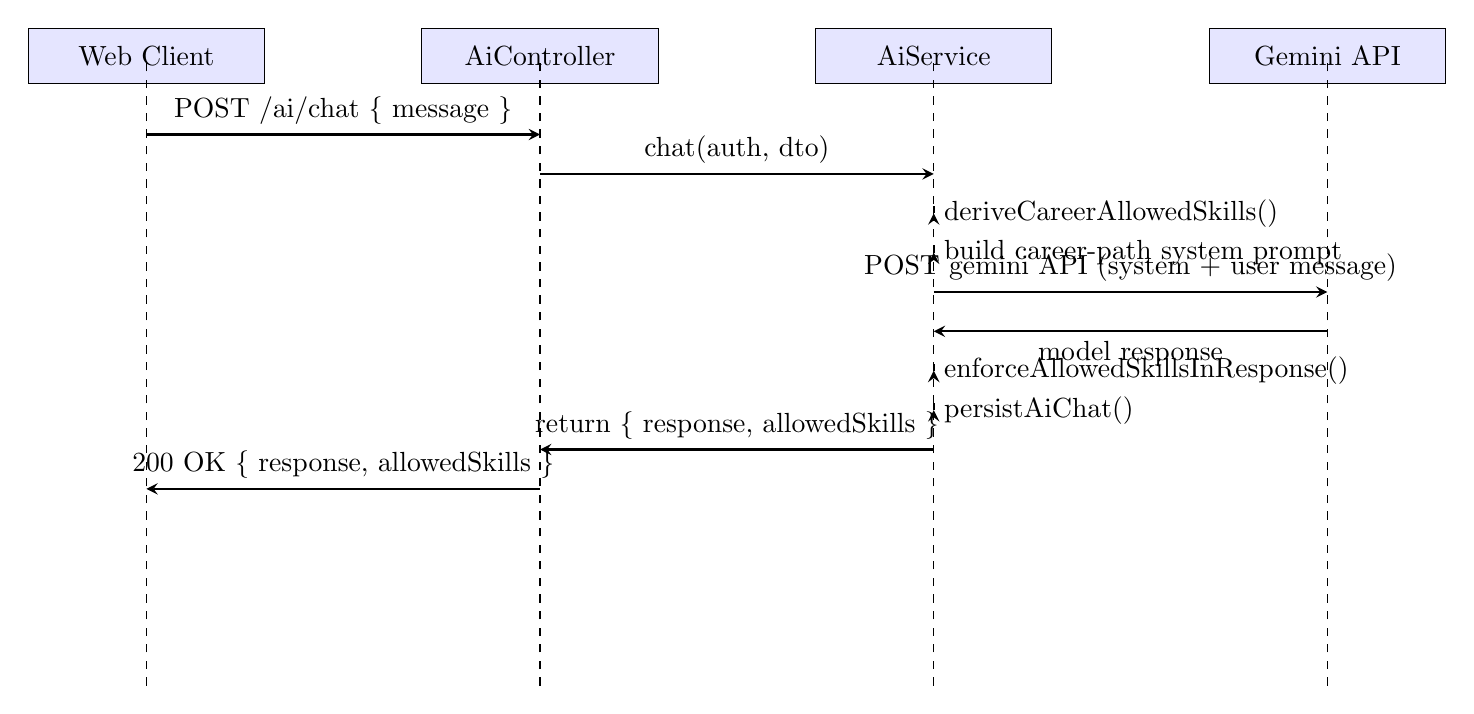
\begin{tikzpicture}[
    lifeline/.style={rectangle, draw, minimum width=3cm, minimum height=0.7cm, align=center, fill=blue!10},
    msg/.style={->, >=stealth, thick}
]
    \node[lifeline] (client) at (0,8) {Web Client};
    \node[lifeline] (ai) at (5,8) {AiController};
    \node[lifeline] (svc) at (10,8) {AiService};
    \node[lifeline] (gemini) at (15,8) {Gemini API};

    \draw[dashed] (0,0) -- (0,8);
    \draw[dashed] (5,0) -- (5,8);
    \draw[dashed] (10,0) -- (10,8);
    \draw[dashed] (15,0) -- (15,8);

    \draw[msg] (0,7) -- (5,7) node[midway, above] {POST /ai/chat \{ message \}};
    \draw[msg] (5,6.5) -- (10,6.5) node[midway, above] {chat(auth, dto)};
    
    \draw[msg] (10,6) -- (10,6) node[right] {deriveCareerAllowedSkills()};
    \draw[msg] (10,5.5) -- (10,5.5) node[right] {build career-path system prompt};
    
    \draw[msg] (10,5) -- (15,5) node[midway, above] {POST gemini API (system + user message)};
    \draw[msg] (15,4.5) -- (10,4.5) node[midway, below] {model response};
    
    \draw[msg] (10,4) -- (10,4) node[right] {enforceAllowedSkillsInResponse()};
    \draw[msg] (10,3.5) -- (10,3.5) node[right] {persistAiChat()};
    
    \draw[msg] (10,3) -- (5,3) node[midway, above] {return \{ response, allowedSkills \}};
    \draw[msg] (5,2.5) -- (0,2.5) node[midway, above] {200 OK \{ response, allowedSkills \}};
\end{tikzpicture}
\caption{Sequence Diagram — AI Chat with Career-Path Enforcement}
\label{fig:seq5}
\end{figure}

\section{Application of Scrum}

\subsection{Team Organization}
The development team consisted of [N] members organized as follows:

\begin{table}[H]
\centering
\caption{Team Organization}
\begin{tabular}{|l|l|p{6cm}|}
\hline
\textbf{Role} & \textbf{Team Member} & \textbf{Responsibilities} \\
\hline
Scrum Master & [Student 1] & Sprint facilitation, impediment removal, GitHub repo management, stakeholder communication \\
\hline
Product Owner & [Student 2] & Product backlog management, feature prioritization, requirement clarification \\
\hline
Backend Developer & [Student 2, Student 4] & NestJS API development, Prisma schema, database design, AI integration, worker services \\
\hline
Frontend Developer & [Student 3] & Next.js UI development, component design, Tailwind CSS styling, Framer Motion animations, print CSS \\
\hline
DevOps Engineer & [Student 4] & Docker containerization, Kubernetes manifests, CI/CD pipeline, Swagger documentation \\
\hline
AI/ML Specialist & [Student 5] & Gemini/Ollama integration, prompt engineering, CV extraction worker, allowed-skills enforcement \\
\hline
\end{tabular}
\end{table}

\subsection{Workflow Management}
Work was managed through GitHub Projects with the following workflow:

\begin{enumerate}[label=\textbf{W-\arabic*}:, leftmargin=*]
    \item \textbf{Product Backlog}: All features, bugs, and improvements maintained as GitHub Issues with labels (feature, bug, enhancement, priority: high/medium/low).
    \item \textbf{Sprint Planning}: At the start of each sprint, the team selected backlog items based on priority and estimated effort, creating a Sprint Backlog.
    \item \textbf{Daily Stand-ups}: 15-minute daily meetings to report progress, plans, and blockers. Conducted via Discord/WhatsApp.
    \item \textbf{Sprint Reviews}: Demo of completed features to the supervisor at the end of each sprint for feedback.
    \item \textbf{Sprint Retrospectives}: Team reflection on what went well, what could be improved, and action items for the next sprint.
    \item \textbf{Git Workflow}: Feature branches (\texttt{feature/auth}, \texttt{feature/resume-templates}) merged to \texttt{main} via Pull Requests with code review.
\end{enumerate}

\subsection{Conflict Resolution}
Conflicts encountered during development included:

\begin{itemize}
    \item \textbf{Technical disagreements on architecture}: Resolved by evaluating options against non-functional requirements (performance, maintainability) and selecting the approach that best met project objectives.
    \item \textbf{Code merge conflicts}: Resolved through pair programming sessions where conflicting developers collaboratively merged changes.
    \item \textbf{Resource constraints (API keys, rate limits)}: Addressed by implementing fallback mechanisms (Gemini → Ollama Cloud) and documenting setup steps clearly.
\end{itemize}

\subsection{Challenges encountered and how they were overcome}

\begin{longtable}{|p{0.5cm}|p{4.5cm}|p{4cm}|p{4cm}|}
\hline
\textbf{\#} & \textbf{Challenge} & \textbf{Impact} & \textbf{Solution} \\
\hline
1 & Docker build failing due to TypeScript compilation errors (CvWizardDataDto not assignable to Prisma JSON types) & Blocked API container deployment & Added \texttt{as Prisma.InputJsonValue} cast with JSON serialization to convert class instances to plain objects \\
\hline
2 & API container restart loop — "prisma: not found" & API unavailable & Changed Dockerfile CMD to use workspace-relative prisma CLI path \\
\hline
3 & Database tables not created — migrate deploy exits 0 with no migrations & All endpoints returning P2021 errors & Switched to \texttt{prisma db push} with \texttt{--accept-data-loss} for schema synchronization \\
\hline
4 & CV scan worker disabled — CV\_SCAN\_ENABLED missing from .env & CV uploads hung indefinitely (8+ minutes) & Added \texttt{CV\_SCAN\_ENABLED="true"} to .env with 30-second overall job timeout \\
\hline
5 & Gemini API key invalid (403 PERMISSION\_DENIED) & CV scan failed & Restored Ollama Cloud fallback for 403 errors and timeouts \\
\hline
6 & MinIO bucket "resumes" not created & Photo uploads failed with "bucket does not exist" & Created bucket via \texttt{mc mb local/resumes} and set anonymous download policy \\
\hline
7 & Print PDF downloading entire dashboard page instead of resume & Resume export broken & Added \texttt{import './print.css'} with @media print rules hiding all non-resume elements \\
\hline
8 & Profile photo not displaying in resume templates & Image broken in templates & Added \texttt{buildMinioUrl()} method to convert object keys to full MinIO URLs \\
\hline
\end{longtable}

\section{Scrum Artifacts}

\subsection{Product Backlog (High-Level Epics)}

\begin{longtable}{|p{0.8cm}|p{3.5cm}|p{3.5cm}|p{1.5cm}|p{1.5cm}|}
\hline
\textbf{ID} & \textbf{Epic / Feature} & \textbf{Description} & \textbf{Priority} & \textbf{Status} \\
\hline
PB-01 & User Authentication & Register, OTP verify, login, JWT refresh, password reset, deactivation & High & Done \\
\hline
PB-02 & Profile Management & Personal details, CV wizard, education, experience CRUD & High & Done \\
\hline
PB-03 & CV Upload \& AI Scan & PDF/DOCX upload to MinIO, BullMQ job queue, Gemini/Ollama text extraction & High & Done \\
\hline
PB-04 & Resume Builder & 6 visual templates, profile data integration, print-to-PDF export, template gallery & High & Done \\
\hline
PB-05 & Job Listings \& Matching & Job browse with search/pagination, AI reranking, job applications & High & Done \\
\hline
PB-06 & AI Chat \& Interview & Career-path restricted chat, mock interviews, course recommendations & High & Done \\
\hline
PB-07 & Mentor Discovery & Mentor profiles, search by skills/expertise & Medium & Done \\
\hline
PB-08 & Real-Time Messaging & Conversations, messages, typing indicators via Socket.IO + Redis & Medium & Done \\
\hline
PB-09 & Video Calling & Agora token generation, session management, mock interview UI & Medium & Done \\
\hline
PB-10 & Notifications & CRUD, mark-read, worker-driven notification fanout & Medium & Done \\
\hline
PB-11 & Admin Dashboard & User management, feedback moderation, analytics KPIs & Medium & Done \\
\hline
PB-12 & Security Hardening & Rate limiting, helmet headers, CORS, RBAC guard, input validation & High & Done \\
\hline
PB-13 & Infrastructure & Docker Compose, Kubernetes manifests, Swagger docs & Medium & Done \\
\hline
\end{longtable}

\subsection{Sprint Backlog (Example: Sprint 2)}

\begin{longtable}{|p{0.8cm}|p{4cm}|p{3cm}|p{2cm}|p{1.5cm}|p{1.5cm}|}
\hline
\textbf{ID} & \textbf{Task} & \textbf{Assignee} & \textbf{Est. (h)} & \textbf{Status} & \textbf{Commit} \\
\hline
SB-01 & Implement Profile CRUD endpoints (GET/PUT /profile) & Backend Dev & 4 & Done & a1b2c3d \\
\hline
SB-02 & Implement Education CRUD endpoints & Backend Dev & 4 & Done & e4f5g6h \\
\hline
SB-03 & Implement Work Experience CRUD endpoints & Backend Dev & 3 & Done & i7j8k9l \\
\hline
SB-04 & Build Profile page UI with form sections & Frontend Dev & 6 & Done & m0n1o2p \\
\hline
SB-05 & Add CvWizardDataDto with validation & Backend Dev & 2 & Done & q3r4s5t \\
\hline
SB-06 & Integrate file upload for profile picture & Frontend + Backend & 4 & Done & u6v7w8x \\
\hline
SB-07 & Add client-side phone validation & Frontend Dev & 2 & Done & y9z0a1b \\
\hline
SB-08 & Add success/error toast notifications & Frontend Dev & 3 & Done & c2d3e4f \\
\hline
\end{longtable}

\section{Test Case Document}

\begin{longtable}{|p{0.7cm}|p{3cm}|p{3.5cm}|p{2.5cm}|p{2.5cm}|}
\hline
\textbf{ID} & \textbf{Test Case} & \textbf{Steps} & \textbf{Expected Result} & \textbf{Actual Result} \\
\hline
TC-01 & Register with valid data & POST /auth/register with email + password & Returns message, OTP logged & Pass \\
\hline
TC-02 & Register with invalid email & POST /auth/register with "notanemail" & Returns 400 Bad Request & Pass \\
\hline
TC-03 & Register with short password & POST /auth/register with \texttt{password: "123"} & Returns 400 Bad Request & Pass \\
\hline
TC-04 & Login after OTP verification & POST /auth/login with verified credentials & Returns accessToken + refreshToken & Pass \\
\hline
TC-05 & Login with wrong password & POST /auth/login with incorrect password & Returns 401 Unauthorized & Pass \\
\hline
TC-06 & Access protected route without token & GET /profile without Authorization header & Returns 401 Unauthorized & Pass \\
\hline
TC-07 & Access protected route with valid token & GET /profile with valid Bearer token & Returns profile data & Pass \\
\hline
TC-08 & Refresh token rotation & POST /auth/refresh with valid refreshToken & Returns new accessToken + refreshToken & Pass \\
\hline
TC-09 & Upload profile picture (valid) & POST /upload/picture with JPEG < 5MB & Returns objectKey, stored in MinIO & Pass \\
\hline
TC-10 & Upload CV (PDF) & POST /upload/cv with valid PDF < 10MB & Returns message, enqueues scan job & Pass \\
\hline
TC-11 & Generate resume (Classic) & POST /resume/build \{template: "CLASSIC"\} & Returns structured resume JSON & Pass \\
\hline
TC-12 & Send message in conversation & POST /conversations/:id/messages & Returns message, broadcasts via Socket.IO & Pass \\
\hline
TC-13 & AI chat — career topic & POST /ai/chat with career question & Returns AI response with allowedSkills & Pass \\
\hline
TC-14 & AI chat — off-topic & POST /ai/chat with non-career question & Returns refusal message & Pass \\
\hline
TC-15 & Admin: view dashboard KPIs & GET /admin/analytics/dashboard (admin token) & Returns activeJobs, totalMentors, aiChats, totalUsers & Pass \\
\hline
TC-16 & Rate limiting — 5 logins/min & POST /auth/login 6 times in 1 minute & 6th request returns 429 Too Many Requests & Pass \\
\hline
TC-17 & Phone validation & PUT /profile with invalid phone format & Returns 400 with validation message & Pass \\
\hline
TC-18 & URL validation (website) & PUT /profile with invalid website URL & Returns 400 with "Invalid website URL" & Pass \\
\hline
TC-19 & File size limit — picture > 5MB & POST /upload/picture with 6MB JPEG & Returns 400 error & Pass \\
\hline
TC-20 & Swagger docs accessible & GET /api-docs & Returns Swagger UI HTML page & Pass \\
\hline
\end{longtable}

\section{Proposed Algorithms}

\subsection{CV Text Extraction and Structured Parsing Algorithm}

\begin{lstlisting}[language=Python, caption={CV Scan Pipeline (Pseudocode)}, label={lst:cvscan}]
function processCvScan(uploadMediaId: string, objectKey: string):
    // Step 1: Download file from MinIO
    buffer = minio.getObject(bucket, objectKey)
    
    // Step 2: Extract raw text based on file type
    if objectKey ends with ".docx":
        rawText = mammoth.extractRawText(buffer)
    else:
        rawText = pdfParse(buffer)
    
    // Step 3: Send to Gemini AI for structured extraction
    prompt = "Extract structured data from CV: {fullName, education[], experience[], skills[], summary}"
    response = gemini.generateContent(prompt + rawText)
    
    // Step 4: Parse JSON response
    structuredData = JSON.parse(response)
    
    // Step 5: Validate and store
    if validate(structuredData):
        update database status = COMPLETED
        store cvExtractedText = JSON.stringify(structuredData)
    else:
        update database status = FAILED
\end{lstlisting}

\subsection{AI Career-Path Enforcement Algorithm}

\begin{lstlisting}[language=Python, caption={Allowed Skills Enforcement (Pseudocode)}, label={lst:allowed}]
function enforceAllowedSkillsInResponse(response: string, allowedSkills: string[]):
    // Split response into words/sentences
    // Check if any allowed skill is mentioned in the response
    for each skill in allowedSkills:
        if response.toLowerCase() contains skill.toLowerCase():
            return response  // Pass — skill mentioned
    
    // If no allowed skill found, refuse the response
    return "I can only discuss career-path skills and topics. Please rephrase your question."
\end{lstlisting}

\subsection{Job Reranking by Skill Relevance}

\begin{lstlisting}[language=Python, caption={Job Reranking Algorithm (Pseudocode)}, label={lst:rerank}]
function rerankJobs(userSkills: string[], jobList: Job[]):
    scored = []
    for each job in jobList:
        score = 0
        for each skill in userSkills:
            if skill in job.skills:
                score += 1
        // Bonus for exact title match
        if userHasJobTitle(job.title):
            score += 2
        scored.push({ job, score })
    
    // Sort descending by score
    scored.sort(by score descending)
    
    // Return top N results with match explanations
    return scored.slice(0, limit).map(item => ({
        ...item.job,
        matchScore: item.score,
        reason: `Matches ${item.score} of your skills`
    }))
\end{lstlisting}

\section{Materials and Technologies Used}

\begin{longtable}{|p{3.5cm}|p{3.5cm}|p{5.5cm}|}
\hline
\textbf{Technology / Material} & \textbf{Category} & \textbf{Role in the System} \\
\hline
TypeScript 5.7 & Programming Language & Primary language for both frontend and backend; provides static type checking, OOP features (classes, interfaces, inheritance, generics) \\
\hline
NestJS 11 & Backend Framework & Modular server-side framework providing dependency injection, middleware pipeline, guards, interceptors, pipes, and decorators \\
\hline
Next.js 16 (React 18) & Frontend Framework & Server-side rendering, file-based routing, API routes, client components with 'use client' directive \\
\hline
Prisma ORM 6.19 & Database ORM & Type-safe database access with schema-first approach, migrations, and generated client \\
\hline
PostgreSQL 16 & Relational Database & Primary data store for all domain entities (users, profiles, jobs, messages, etc.) \\
\hline
Redis 7 & Cache / Message Broker & BullMQ job queue backend, Socket.IO pub/sub adapter for horizontal scaling, session caching \\
\hline
BullMQ 5 & Job Queue & Asynchronous background processing for CV scanning and notification dispatching \\
\hline
MinIO & Object Storage & S3-compatible storage for profile pictures and CV/resume files \\
\hline
Docker & Containerization & Consistent development and production environments, service isolation \\
\hline
Kubernetes & Orchestration & Production deployment with HPA, stateful sets, ingress, and TLS \\
\hline
Google Gemini API & AI Provider & Natural language generation for AI chat, mock interviews, course recommendations, and structured CV parsing \\
\hline
Ollama Cloud API & AI Fallback & Secondary AI provider used when Gemini returns 403, 429, or times out \\
\hline
Socket.IO 4 & Real-time Communication & Bidirectional WebSocket events for messaging, typing indicators, and online status \\
\hline
Agora Web SDK & Video Calling & Low-latency video/audio for mock interview sessions \\
\hline
Framer Motion 12 & Animation Library & Page transitions, hover effects, scroll animations, toast notifications \\
\hline
Tailwind CSS 3 & CSS Framework & Utility-first responsive styling with custom design tokens \\
\hline
Swagger/OpenAPI & API Documentation & Auto-generated interactive API documentation at /api-docs endpoint \\
\hline
JWT (jsonwebtoken) & Authentication & Stateless access/refresh token generation and verification \\
\hline
bcryptjs & Cryptography & Password hashing with salt rounds for secure credential storage \\
\hline
class-validator & Input Validation & Declarative validation decorators on DTOs (IsEmail, IsUrl, MinLength, Matches) \\
\hline
class-transformer & Data Transformation & JSON-to-class instance conversion with type coercion \\
\hline
Jest 30 & Testing Framework & Unit tests and integration tests for backend services \\
\hline
Supertest 7 & HTTP Testing & End-to-end API testing with request simulation and response assertion \\
\hline
ESLint + Prettier & Code Quality & Static analysis, code formatting, and style enforcement \\
\hline
Git + GitHub & Version Control & Source code management, feature branching, pull request code review \\
\hline
\end{longtable}

\subsection{Object-Oriented Programming Concepts Applied}

\begin{longtable}{|p{2.5cm}|p{4.5cm}|p{5.5cm}|}
\hline
\textbf{OOP Concept} & \textbf{Where Used} & \textbf{Why Used} \\
\hline
\textbf{Encapsulation} & All service classes (AuthService, ProfileService, ResumeService, etc.) & Business logic and data access are encapsulated within service methods. Private helper methods handle internal operations; public methods expose the API contract. DTOs encapsulate validated request data. \\
\hline
\textbf{Inheritance} & RedisIoAdapter extends default Socket.IO adapter & Reuses base WebSocket functionality while adding Redis pub/sub synchronization for multi-instance deployment. NestJS interceptors extend base class behavior. \\
\hline
\textbf{Polymorphism} & UploadService.uploadToMinio() handles both PROFILE\_PICTURE and CV types via MediaType enum & Single method processes different upload types with type-specific logic. ResumeService.formatResume() renders 6 different templates through a common data interface. \\
\hline
\textbf{Abstraction} & PrismaService abstracts database operations; DTOs abstract request validation; AIProvider abstracts Gemini/Ollama provider selection & Hides implementation complexity behind clean interfaces. Consumers don't need to know Prisma query syntax or AI provider details. \\
\hline
\textbf{Dependency Injection} & NestJS DI container injects PrismaService, CvScanService, etc. into controllers and services & Decouples components for testability and maintainability. Services can be mocked in unit tests. \\
\hline
\textbf{Interfaces} & ResumeData TypeScript interface, CvWizardData contract, BullMqQueueLike interface & Define clear contracts between components. The CV scan worker interacts with BullMQ through an interface, making it swappable. \\
\hline
\textbf{Generics} & apiFetch<T>() in frontend, Prisma type generics, class-validator generic decorators & Type-safe API calls and database queries. Prevents runtime type errors at compile time. \\
\hline
\end{longtable}

\subsection{Use of Swagger for API Documentation Automation}

The Career Navigator project uses NestJS's native Swagger/OpenAPI integration to automatically generate comprehensive API documentation. The configuration is in \texttt{apps/api/src/main.ts}:

\begin{itemize}
    \item \textbf{DocumentBuilder API}: Programmatically constructs the OpenAPI specification with title, description, version, server URLs, tags, and bearer authentication scheme.
    \item \textbf{Bearer Auth}: The \texttt{addBearerAuth()} configuration enables the "Authorize" button in Swagger UI. Users can paste their JWT access token to test protected endpoints interactively.
    \item \textbf{Automatic Schema Generation}: NestJS reflects on TypeScript types and \texttt{class-validator} decorators (e.g., \texttt{@IsEmail}, \texttt{@IsString}, \texttt{@MinLength}) to generate request/response schemas automatically. No manual schema writing is required.
    \item \textbf{Controller Decorators}: \texttt{@ApiTags()} groups endpoints by domain (auth, profile, jobs, etc.). \texttt{@ApiOkResponse()}, \texttt{@ApiUnauthorizedResponse()}, and \texttt{@ApiBadRequestResponse()} document expected response codes.
    \item \textbf{UI Configuration}: \texttt{persistAuthorization: true} keeps the token after page refresh. \texttt{filter: true} adds a search bar. \texttt{tryItOutEnabled: true} enables the "Try it out" button on every endpoint.
    \item \textbf{Access}: The documentation is served at \texttt{http://localhost:3001/api-docs} when the API is running.
\end{itemize}

% ============================================================
% CHAPTER FOUR: RESULTS AND DISCUSSIONS
% ============================================================
\chapter{Results and Discussions}

\section{Screenshots of Application Scenarios}

\subsection{Authentication Screens}

\begin{figure}[H]
\centering
\fbox{\parbox{0.7\textwidth}{\centering
    \vspace{3cm}
    \textbf{[Screenshot: Login Page]}\\
    Login form with email/password fields,\\
    "Forgot password?" link, Register link\\
    \vspace{3cm}
}}
\caption{Login Page}
\end{figure}

\begin{figure}[H]
\centering
\fbox{\parbox{0.7\textwidth}{\centering
    \vspace{3cm}
    \textbf{[Screenshot: Register Page]}\\
    Registration form with email, password,\\
    confirm password, and OTP verification step\\
    \vspace{3cm}
}}
\caption{Registration Page}
\end{figure}

\subsection{Profile Management}

\begin{figure}[H]
\centering
\fbox{\parbox{0.7\textwidth}{\centering
    \vspace{3cm}
    \textbf{[Screenshot: Profile Page]}\\
    Profile form with sections: Professional Identity,\\
    Profile Photo (file upload), Personal Details,\\
    CV Sections (skills, languages, interests),\\
    Education and Experience inline forms\\
    \vspace{3cm}
}}
\caption{Profile Management Page}
\end{figure}

\subsection{Resume Builder}

\begin{figure}[H]
\centering
\fbox{\parbox{0.7\textwidth}{\centering
    \vspace{3cm}
    \textbf{[Screenshot: Resume Builder Page]}\\
    6 template cards (Classic, Modern, Minimal,\\
    Creative, Professional, Executive),\\
    resume preview with template rendering,\\
    "Download as PDF" button\\
    \vspace{3cm}
}}
\caption{Resume Builder with Template Selection}
\end{figure}

\subsection{AI Chat Interface}

\begin{figure}[H]
\centering
\fbox{\parbox{0.7\textwidth}{\centering
    \vspace{3cm}
    \textbf{[Screenshot: AI Chat Page]}\\
    Chat interface with message history,\\
    career-path restricted responses,\\
    skill tags display\\
    \vspace{3cm}
}}
\caption{AI Chat Interface}
\end{figure}

\subsection{Admin Dashboard}

\begin{figure}[H]
\centering
\fbox{\parbox{0.7\textwidth}{\centering
    \vspace{3cm}
    \textbf{[Screenshot: Admin Analytics Dashboard]}\\
    KPI cards: Active Jobs, Total Mentors,\\
    AI Chats count, Total Users\\
    \vspace{3cm}
}}
\caption{Admin Analytics Dashboard}
\end{figure}

\section{API Request/Response Examples (Swagger)}

\subsection{POST /auth/register}

\textbf{Request:}
\begin{lstlisting}[language=json]
{
  "email": "student@university.edu",
  "password": "SecurePass123!"
}
\end{lstlisting}

\textbf{Response (200 OK):}
\begin{lstlisting}[language=json]
{
  "message": "OTP sent to your email for verification."
}
\end{lstlisting}

\subsection{POST /auth/login}

\textbf{Request:}
\begin{lstlisting}[language=json]
{
  "email": "student@university.edu",
  "password": "SecurePass123!"
}
\end{lstlisting}

\textbf{Response (200 OK):}
\begin{lstlisting}[language=json]
{
  "accessToken": "eyJhbGciOiJIUzI1NiIs...",
  "refreshToken": "dGhpcyBpcyBhIHJlZnJl..."
}
\end{lstlisting}

\subsection{POST /resume/build}

\textbf{Request:}
\begin{lstlisting}[language=json]
{
  "template": "MODERN"
}
\end{lstlisting}

\textbf{Response (200 OK):}
\begin{lstlisting}[language=json]
{
  "template": "MODERN",
  "sections": {
    "header": {
      "fullName": "John Doe",
      "headline": "Software Engineer",
      "contact": { "phone": "+234...", "email": "john@..." }
    },
    "skills": ["React", "Node.js", "TypeScript"],
    "experience": [...],
    "education": [...],
    "projects": [...],
    "references": [...]
  }
}
\end{lstlisting}

\subsection{POST /ai/chat}

\textbf{Request:}
\begin{lstlisting}[language=json]
{
  "message": "What skills should I learn for a career in cloud computing?"
}
\end{lstlisting}

\textbf{Response (200 OK):}
\begin{lstlisting}[language=json]
{
  "response": "For a career in cloud computing, focus on...",
  "allowedSkills": ["AWS", "Azure", "Docker", "Kubernetes", "Terraform"]
}
\end{lstlisting}

\subsection{GET /admin/analytics/dashboard}

\textbf{Response (200 OK):}
\begin{lstlisting}[language=json]
{
  "activeJobs": 45,
  "totalMentors": 12,
  "aiChats": 238,
  "totalUsers": 156
}
\end{lstlisting}

\subsection{Swagger UI Screenshot}

\begin{figure}[H]
\centering
\fbox{\parbox{0.8\textwidth}{\centering
    \vspace{4cm}
    \textbf{[Screenshot: Swagger UI at /api-docs]}\\
    Interactive API documentation with all endpoints\\
    grouped by tags (auth, profile, resume, jobs, etc.),\\
    "Authorize" button for JWT token input,\\
    "Try it out" functionality for each endpoint\\
    \vspace{4cm}
}}
\caption{Swagger/OpenAPI Documentation UI}
\end{figure}

% ============================================================
% CHAPTER FIVE: RECOMMENDATIONS AND CONCLUSION
% ============================================================
\chapter{Recommendations and Conclusion}

\section{Conclusion}

The Career Navigator project has successfully delivered a comprehensive, AI-enhanced career development platform that integrates profile management, automated resume building with six professional templates, AI-powered CV scanning and skill extraction, job matching with relevance scoring, mentor discovery, real-time messaging, video calling for mock interviews, and an administrative analytics dashboard — all within a single, unified web application.

The system was developed using modern software engineering practices: a NestJS (TypeScript) modular backend with Prisma ORM and PostgreSQL persistence, a Next.js (React/TypeScript) frontend with Tailwind CSS and Framer Motion animations, containerized via Docker and orchestrated with Kubernetes manifests. The Scrum agile methodology guided the development process through eight sprints, with comprehensive testing (Jest unit tests, Supertest end-to-end tests, and 20 manual test cases) ensuring quality across all 30 functional requirements and 10 non-functional requirements.

Key technical achievements include: implementation of secure JWT authentication with access/refresh token rotation and OTP email verification; integration of Google Gemini and Ollama Cloud AI providers with career-path content enforcement; development of a BullMQ-based asynchronous CV scanning pipeline with automatic fallback; creation of six distinct A4 resume templates with print-to-PDF export; real-time messaging via Socket.IO with Redis pub/sub for horizontal scaling; and automated API documentation generation via Swagger/OpenAPI.

Object-oriented programming principles were rigorously applied throughout the codebase: encapsulation in service classes, inheritance in adapter extensions, polymorphism in multi-type upload handling and template rendering, abstraction through PrismaService and DTOs, dependency injection via NestJS's IoC container, interfaces defining clear component contracts, and TypeScript generics ensuring type safety.

The project demonstrates the effective application of full-stack web development, cloud-native architecture patterns, AI/ML integration, and agile project management to solve a real-world problem in career development and educational technology.

\section{Difficulties Encountered}

During the development of Career Navigator, the team encountered several significant challenges. Docker containerization proved particularly demanding, with TypeScript compilation errors blocking API container builds and requiring iterative debugging of Prisma type compatibility. The CV scanning pipeline presented persistent difficulties: the worker service was initially disabled due to a missing environment variable, the Gemini API key was invalid (returning HTTP 403), and the absence of an overall job timeout caused uploads to hang indefinitely. These issues were progressively resolved through environment configuration, API key management, fallback mechanisms, and the addition of a 30-second job timeout. Infrastructure configuration challenges included MinIO bucket provisioning (the "resumes" bucket had to be manually created and made publicly readable) and print CSS styling for the resume PDF export (initially printing the entire dashboard page instead of just the template). Coordination between frontend and backend development, especially around the cvWizardData JSON serialization (class-transformer instances vs. plain objects for Prisma), required careful debugging and close collaboration.

\section{Recommendations for Further Studies}

Future work on the Career Navigator platform should focus on several key areas for enhancement. First, the AI capabilities could be significantly expanded by integrating a dedicated large language model fine-tuned on career counseling data, improving the quality and specificity of career guidance, mock interviews, and skill gap analysis. Second, the recommendation engine should be enhanced with collaborative filtering and content-based machine learning models to provide personalized job and mentor recommendations based on user behavior patterns and success metrics. Third, mobile applications for iOS and Android should be developed using React Native (leveraging the existing React codebase) to improve accessibility for users in regions where mobile devices are the primary computing platform. Fourth, the platform should incorporate a skills assessment module with coding challenges, aptitude tests, and personality assessments to provide a more holistic career profile. Fifth, integration with university learning management systems (LMS) via LTI standards would enable automatic population of academic records and course histories. Sixth, advanced analytics including career trajectory prediction, labor market trend analysis, and salary benchmarking would provide additional value to users. Finally, multilingual support should be implemented to serve non-English speaking populations, particularly in African and Asian markets where career guidance platforms are most needed.

\end{document}
